\documentclass[11pt,a4paper]{article}
\usepackage{fontspec}
\setmainfont{TeX Gyre Termes}
\setmonofont{Latin Modern Mono}[Scale=0.95]
\usepackage[margin=2.6cm,top=2.8cm,bottom=2.8cm]{geometry}
\usepackage{graphicx,booktabs,amsmath,xcolor,listings,fancyhdr,caption,titlesec,microtype,enumitem,tikz}
\usetikzlibrary{positioning,arrows.meta}
\usepackage[hidelinks]{hyperref}
\usepackage{float}

\definecolor{codebg}{HTML}{F5F5F2}
\definecolor{codekw}{HTML}{1C5CAB}
\definecolor{codecm}{HTML}{6E6D68}
\definecolor{accent}{HTML}{2A78D6}
\definecolor{ink}{HTML}{2B2B2B}
\lstset{basicstyle=\ttfamily\small,backgroundcolor=\color{codebg},
  keywordstyle=\color{codekw},commentstyle=\color{codecm}\itshape,
  frame=none,xleftmargin=1em,framexleftmargin=1em,aboveskip=8pt,belowskip=4pt,
  columns=fullflexible,keepspaces=true,showstringspaces=false,
  numbers=left,numberstyle=\tiny\color{codecm},numbersep=6pt}
\lstdefinestyle{py}{language=Python}
\lstdefinestyle{r}{language=R}
\lstdefinestyle{sql}{language=SQL,morekeywords={ROUND,CASE,WHEN,THEN,ELSE,END,HAVING}}

% "Code:" reference line printed under each figure, table and listing
\newcommand{\coderef}[1]{\par\vspace{2pt}{\centering\footnotesize\color{codecm}\textsf{Code:}~\texttt{#1}\par}}
\newcommand{\file}[1]{\texttt{#1}}

\captionsetup{font={small,it},labelfont={small,it},justification=centering}
\titleformat{\section}{\large\bfseries}{\thesection.}{0.5em}{}
\titleformat{\subsection}{\normalsize\bfseries}{\thesubsection}{0.5em}{}
\titlespacing*{\section}{0pt}{14pt}{6pt}
\titlespacing*{\subsection}{0pt}{10pt}{4pt}
\setlength{\parskip}{5pt}\setlength{\parindent}{0pt}

\pagestyle{fancy}\fancyhf{}
\fancyhead[L]{\small\itshape Credit Risk in Germany: Technical Companion}
\fancyhead[R]{\small\itshape Ettore Mancuso}
\fancyfoot[C]{\small\thepage}
\renewcommand{\headrulewidth}{0.4pt}\renewcommand{\footrulewidth}{0.4pt}

\begin{document}
\thispagestyle{empty}
\begin{center}
{\LARGE\bfseries Credit Risk in Germany\\[4pt] Technical Companion}\\[10pt]
{\large\itshape How the analysis was built: data, code and design choices,\\ step by step}\\[22pt]
{\large Ettore Mancuso}\\[1pt]
\href{mailto:ettoremancuso6@gmail.com}{ettoremancuso6@gmail.com}\\[1pt]
October 2026
\end{center}
\vspace{12pt}

\section*{Why this document}
The paper \textit{Credit Risk in Germany: From System-Wide Signals to a Borrower-Level PD Model} reports results. This companion shows how I got them. It follows the same order as the analysis, and under every chart, table and code excerpt there is a \textsf{Code:} line that points to the exact file, notebook cell or function that produced it, so anyone can open the repository and find it in a few seconds.

I wrote it mainly for people who want to judge the programming side of the project. In short: the analysis is a single Python notebook that runs from start to finish in well under a minute, the reusable logic sits in two small modules, SQL handles the segment analysis, an R script cross-checks the main model, and every output is exported as CSV for a Power BI report. Notebook cells are cited by their execution number, \texttt{[n]}, as shown in Jupyter.

\begin{table}[H]\centering\small
\caption{Tools used and what each one does in the project.}\label{tab:tools}
\begin{tabular}{p{2.6cm}p{4.6cm}p{6.4cm}}
\toprule
Tool & Libraries / setup & Role \\
\midrule
Python 3 & pandas, NumPy, SciPy & Data handling, numerical root finding (\texttt{brentq}), normal distribution for the capital formula \\
 & scikit-learn & Train/test split, cross-validation, random forest, gradient boosting, ROC/AUC \\
 & statsmodels & Unpenalised logit with standard errors and p-values \\
 & matplotlib & All six figures (exported as vector PDF and PNG) \\
SQL & SQLite (in memory) & Default rates by segment, queries kept in a separate \file{.sql} file \\
R & base R (\texttt{glm}) & Independent cross-check of the logistic model on the same split \\
Jupyter & nbconvert & Main analysis notebook, also executable from the command line \\
 & pytest, GitHub Actions & Unit tests for the two modules, run automatically on every push \\
Power BI & CSV exports & Reporting layer built on \file{outputs/} \\
\LaTeX\ & XeLaTeX & Paper and this companion \\
Git / GitHub & & Version control and publication \\
\bottomrule
\end{tabular}
\end{table}

\section{Architecture of the repository}
Figure~\ref{fig:pipe} shows how data move through the project. Raw inputs never change; everything downstream can be deleted and rebuilt by running the notebook.

\begin{figure}[H]\centering
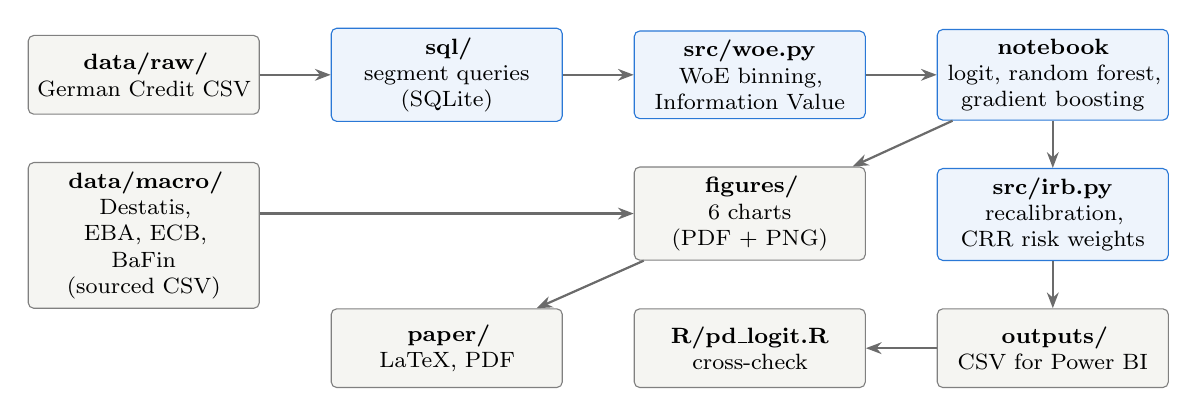
\begin{tikzpicture}[
  box/.style={draw=ink!60, rounded corners=2pt, fill=codebg, align=center, font=\footnotesize, minimum height=10mm, text width=27mm},
  hl/.style={box, draw=accent, fill=accent!8},
  arr/.style={-{Stealth[length=2mm]}, ink!70, thick}]
\node[box] (raw) {\textbf{data/raw/}\\German Credit CSV};
\node[box, below=6mm of raw] (macro) {\textbf{data/macro/}\\Destatis, EBA, ECB,\\BaFin (sourced CSV)};
\node[hl, right=9mm of raw] (sql) {\textbf{sql/}\\segment queries\\(SQLite)};
\node[hl, right=9mm of sql] (woe) {\textbf{src/woe.py}\\WoE binning,\\Information Value};
\node[hl, right=9mm of woe] (models) {\textbf{notebook}\\logit, random forest,\\gradient boosting};
\node[hl, below=6mm of models] (irb) {\textbf{src/irb.py}\\recalibration,\\CRR risk weights};
\node[box, below=6mm of woe] (fig) {\textbf{figures/}\\6 charts\\(PDF + PNG)};
\node[box, below=6mm of irb] (out) {\textbf{outputs/}\\CSV for Power BI};
\node[box, left=9mm of out] (r) {\textbf{R/pd\_logit.R}\\cross-check};
\node[box, left=9mm of r] (paper) {\textbf{paper/}\\LaTeX, PDF};
\draw[arr] (raw) -- (sql);
\draw[arr] (sql) -- (woe);
\draw[arr] (woe) -- (models);
\draw[arr] (models) -- (irb);
\draw[arr] (irb) -- (out);
\draw[arr] (macro.east |- fig.west) -- (fig.west);
\draw[arr] (models) -- (fig);
\draw[arr] (out) -- (r);
\draw[arr] (fig) -- (paper);
\end{tikzpicture}
\caption{Data flow through the repository. Blue boxes contain the analytical code.}\label{fig:pipe}
\coderef{README.md (repository map)}
\end{figure}

Three choices shaped the structure:

\begin{itemize}[leftmargin=1.5em,itemsep=2pt]
\item \textbf{Logic in modules, story in the notebook.} Functions that I might reuse (WoE encoding, the capital formula) live in \file{src/} and are imported by the notebook. The notebook only calls them and shows results.
\item \textbf{One source per number.} Every hand-collected value has a \texttt{source} column next to it, so a reader can check any figure in the paper against its origin.
\item \textbf{Reproducible by default.} A fixed random seed (\texttt{SEED = 42}), relative paths and a list of required packages. I tested this by copying the repository to an empty folder, deleting all outputs and running everything again: the results were identical.
\end{itemize}

\section{Step 1: collecting and checking system-level data}
Public banking statistics are scattered across institutions and change definition over time, so I collected the values by hand into three small CSV files. Each row records where the number comes from. The notebook loads them with pandas and computes the derived figures quoted in the paper, such as the change in insolvencies from the 2021 trough.

\par\noindent\begin{minipage}{\linewidth}
\begin{lstlisting}[style=py]
ins = pd.read_csv(ROOT / "data/macro/insolvencies_de.csv")
npl = pd.read_csv(ROOT / "data/macro/npl_indicators.csv", parse_dates=["date"])
ins["yoy_pct"] = ins.corporate_insolvencies.pct_change() * 100
low = ins.loc[ins.corporate_insolvencies.idxmin()]
last = ins.corporate_insolvencies.iloc[-1]
print(f"2025 vs trough: {last / low.corporate_insolvencies - 1:+.1%}")
\end{lstlisting}
\coderef{notebooks/german\_credit\_risk.ipynb, cell [2] (Python, pandas)}
\end{minipage}\par

A simple consistency check caught a gap early: Destatis's historical table stops in 2022, and the 2023 and 2024 values come from press releases. I verified that the reported growth rates (+22.1\% and +22.4\%) reproduce the levels before accepting them.

\begin{figure}[H]\centering
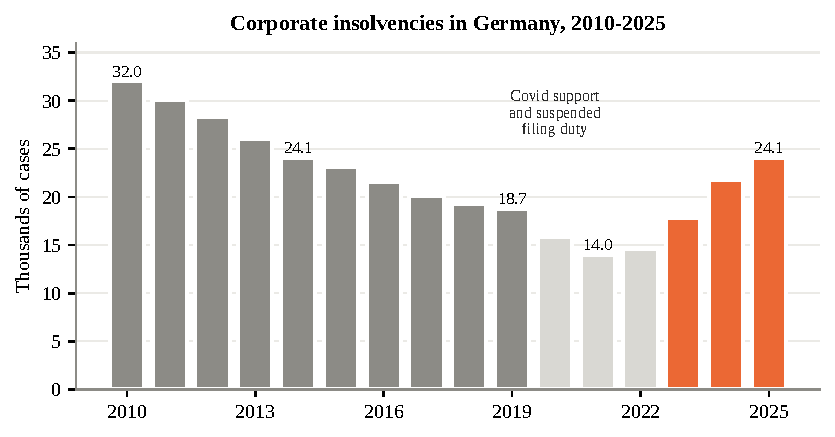
\includegraphics[width=0.80\textwidth]{../figures/fig1_insolvencies.pdf}
\caption{Corporate insolvencies in Germany, 2010--2025 (paper, Figure 1).}
\coderef{notebooks/german\_credit\_risk.ipynb, cell [3] (Python, matplotlib) \textbar{} data: data/macro/insolvencies\_de.csv}
\end{figure}

For the EU comparison I used a dumbbell chart: one row per indicator, with Germany and the EU joined by a line, so the size and the direction of the gap are visible at once.

\begin{figure}[H]\centering
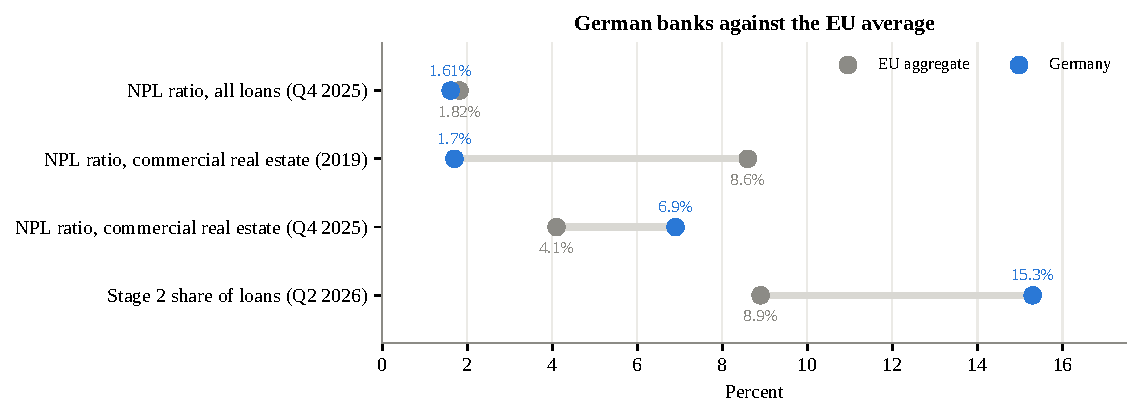
\includegraphics[width=0.80\textwidth]{../figures/fig2_npl_compare.pdf}
\caption{German banks against the EU average (paper, Figure 2).}
\coderef{notebooks/german\_credit\_risk.ipynb, cell [4] (Python, matplotlib) \textbar{} data: data/macro/npl\_indicators.csv}
\end{figure}

\section{Step 2: exploring the loan data with SQL}
Before modelling I wanted a feel for the data, and the quickest way to ask ``what is the default rate by group?'' is SQL. The notebook loads the CSV into an in-memory SQLite database. The queries live in their own file, so they can be read, reused or run in any SQL client without opening Python.

\par\noindent\begin{minipage}{\linewidth}
\begin{lstlisting}[style=sql]
SELECT CASE
         WHEN duration_in_month <= 12 THEN '01-12 months'
         WHEN duration_in_month <= 24 THEN '13-24 months'
         WHEN duration_in_month <= 36 THEN '25-36 months'
         ELSE '37+ months'
       END                          AS segment,
       COUNT(*)                     AS n,
       SUM(bad)                     AS defaults,
       ROUND(100.0 * AVG(bad), 1)   AS default_rate_pct,
       ROUND(AVG(credit_amount), 0) AS avg_amount_dm
FROM loans
GROUP BY segment
ORDER BY segment;
\end{lstlisting}
\coderef{sql/segments.sql, query by\_duration\_band (SQL, SQLite)}
\end{minipage}\par

The notebook splits the file on its \texttt{-- name:} markers and runs each query with \texttt{pd.read\_sql}:

\par\noindent\begin{minipage}{\linewidth}
\begin{lstlisting}[style=py]
con = sqlite3.connect(":memory:")
raw.to_sql("loans", con, index=False)
for block in (ROOT / "sql/segments.sql").read_text().split("-- name: ")[1:]:
    name, sql = block.split("\n", 1)
    queries[name.strip()] = sql.strip()
seg = {name: pd.read_sql(q, con) for name, q in queries.items()}
\end{lstlisting}
\coderef{notebooks/german\_credit\_risk.ipynb, cell [6] (Python + SQL)}
\end{minipage}\par

\begin{table}[H]\centering\small
\caption{Output of the duration query.}
\begin{tabular}{lrrrr}
\toprule
Segment & Loans & Defaults & Default rate & Avg. amount (DM) \\
\midrule
01--12 months & 359 & 76 & 21.2\% & 1,811 \\
13--24 months & 411 & 122 & 29.7\% & 2,924 \\
25--36 months & 143 & 57 & 39.9\% & 5,274 \\
37+ months & 87 & 45 & 51.7\% & 7,646 \\
\bottomrule
\end{tabular}
\coderef{sql/segments.sql, executed in notebook cell [6]}
\end{table}

\section{Step 3: feature engineering with Weight of Evidence}
A credit scorecard does not use raw variables. Each one is split into bins, and each bin is replaced by its Weight of Evidence (WoE), the log ratio between the share of good and bad loans that fall in it. This handles categorical and numeric variables in the same way, makes the relation with default monotone, and gives the Information Value (IV), a measure of how much each variable can separate good from bad loans.

I wrote the encoder myself instead of using a package, partly to understand it and partly to control one detail: the bins must be learned on training data only. The class follows the scikit-learn \texttt{fit}/\texttt{transform} pattern.

\par\noindent\begin{minipage}{\linewidth}
\lstinputlisting[style=py,firstline=28,lastline=48,firstnumber=28]{../src/woe.py}
\coderef{src/woe.py, function woe\_table() (Python, pandas)}
\end{minipage}\par

\par\noindent\begin{minipage}{\linewidth}
\lstinputlisting[style=py,firstline=69,lastline=80,firstnumber=69]{../src/woe.py}
\coderef{src/woe.py, method WoEEncoder.fit()}
\end{minipage}\par

Two details are worth pointing out. The smoothing constant of 0.5 (lines 43--44) avoids an infinite WoE when a bin has no defaults. And in \texttt{fit}, the outer bin edges are set to $\pm\infty$ (line 76), so a test value outside the training range still falls into a bin instead of producing a missing value.

\begin{figure}[H]\centering
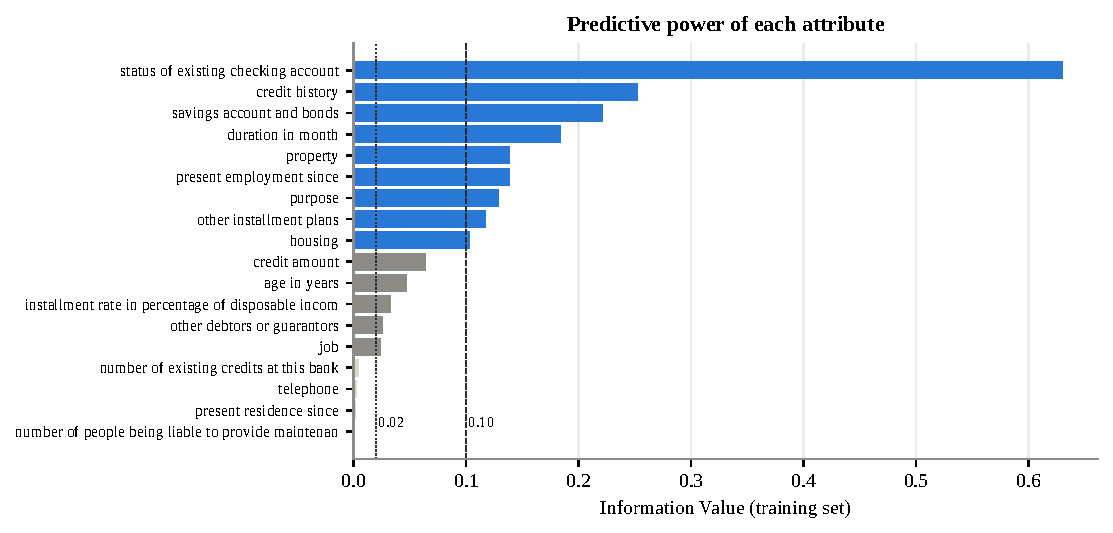
\includegraphics[width=0.80\textwidth]{../figures/fig3_iv.pdf}
\caption{Information Value of each attribute (paper, Figure 3).}
\coderef{notebooks/german\_credit\_risk.ipynb, cells [7] (WoE fit, IV table) and [8] (matplotlib) \textbar{} src/woe.py}
\end{figure}

\section{Step 4: three models and a fair comparison}
I compared a logistic scorecard with two machine-learning models. The main programming issue was \textit{data leakage}: if the WoE bins were fitted on the whole training set before cross-validation, every validation fold would have ``seen'' its own outcomes through the encoding, and the scorecard would look better than it is. To prevent it I wrapped the encoder and the regression in one small class, so that both are refitted inside every fold:

\par\noindent\begin{minipage}{\linewidth}
\begin{lstlisting}[style=py]
class WoELogit:
    """WoE encoding + logistic regression, refitted inside each CV fold."""
    def __init__(self, features): self.features = features
    def fit(self, X, y):
        self.enc = WoEEncoder(5).fit(X[self.features], y)
        self.lr = LogisticRegression(C=1.0, max_iter=1000).fit(
            self.enc.transform(X[self.features]), y)
        return self
    def predict_proba(self, X):
        return self.lr.predict_proba(self.enc.transform(X[self.features]))
\end{lstlisting}
\coderef{notebooks/german\_credit\_risk.ipynb, cell [9] (Python, scikit-learn)}
\end{minipage}\par

The random forest and the gradient boosting model are scikit-learn \texttt{Pipeline}s with one-hot encoding. All three go through the same loop, so the comparison is like for like:

\par\noindent\begin{minipage}{\linewidth}
\begin{lstlisting}[style=py]
skf = StratifiedKFold(n_splits=5, shuffle=True, random_state=SEED)
for name, model in models.items():
    cv_auc = []
    for tr, va in skf.split(X_tr, y_tr):
        m = model.fit(X_tr.iloc[tr], y_tr.iloc[tr])
        cv_auc.append(discrimination(y_tr.iloc[va],
                                     m.predict_proba(X_tr.iloc[va])[:, 1])["AUC"])
    model.fit(X_tr, y_tr)                       # refit on the full training set
    p = model.predict_proba(X_te)[:, 1]         # score the untouched test set
\end{lstlisting}
\coderef{notebooks/german\_credit\_risk.ipynb, cell [9]}
\end{minipage}\par

\begin{table}[H]\centering\small
\caption{Model comparison (paper, Table 2).}
\begin{tabular}{lcccccc}
\toprule
Model & CV AUC & CV s.d. & Test AUC & Gini & KS & Brier \\
\midrule
Logistic scorecard (WoE) & 0.758 & 0.019 & 0.801 & 0.601 & 0.502 & 0.159 \\
Random forest & 0.783 & 0.035 & 0.794 & 0.587 & 0.481 & 0.166 \\
Gradient boosting & 0.764 & 0.019 & 0.796 & 0.592 & 0.462 & 0.159 \\
\bottomrule
\end{tabular}
\coderef{notebooks/german\_credit\_risk.ipynb, cell [9] \textbar{} exported to outputs/model\_comparison.csv}
\end{table}

\begin{figure}[H]\centering
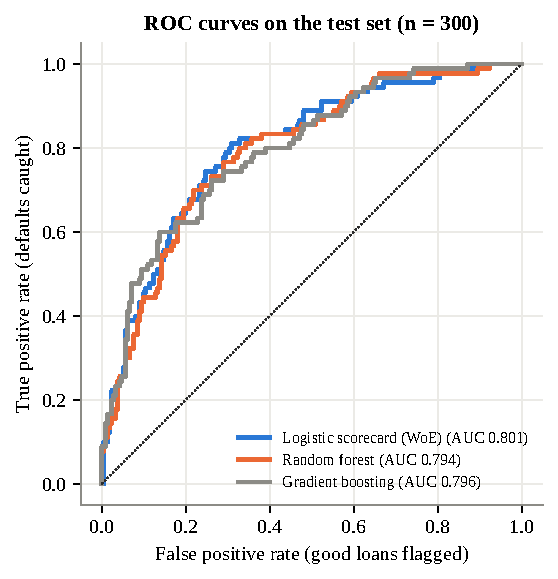
\includegraphics[width=0.55\textwidth]{../figures/fig4_roc.pdf}
\caption{ROC curves on the test set (paper, Figure 4).}
\coderef{notebooks/german\_credit\_risk.ipynb, cell [10] (scikit-learn roc\_curve, matplotlib)}
\end{figure}

\section{Step 5: checking the model from a second angle, in R}
Two checks make me more confident that the scorecard is sound. In Python, statsmodels gives the unpenalised logit with standard errors: 13 of 14 coefficients have the expected sign (cell [11]). In R, I fitted a plain logistic regression on dummy-coded categories. To make the comparison meaningful, the R script reads the exact test rows that Python used, which the notebook saves to \file{outputs/test\_index.csv}. Python indexes from 0 and R from 1, hence the \texttt{+ 1} on line 12.

\par\noindent\begin{minipage}{\linewidth}
\lstinputlisting[style=r,firstline=6,lastline=27,firstnumber=6]{../R/pd_logit.R}
\coderef{R/pd\_logit.R (base R, glm) \textbar{} output: Test AUC 0.792, Gini 0.584}
\end{minipage}\par

The R model reaches a test AUC of 0.792, against 0.801 for the scorecard: a different encoding and a different language, but almost the same answer. I computed the AUC with the Mann--Whitney formula so that the script needs no extra packages.

\section{Step 6: from scores to rating grades}
To place every loan in a grade without in-sample bias, each one is scored by a model trained on the other four fifths of the data (out-of-fold prediction). The PDs are then moved to a realistic 3\% average. The function shifts the log-odds of every loan by the same factor and finds that factor numerically with SciPy's \texttt{brentq}, so the ranking, and therefore the AUC, does not change.

\par\noindent\begin{minipage}{\linewidth}
\lstinputlisting[style=py,firstline=45,lastline=60,firstnumber=45]{../src/irb.py}
\coderef{src/irb.py, function recalibrate() (Python, NumPy, SciPy)}
\end{minipage}\par

\par\noindent\begin{minipage}{\linewidth}
\begin{lstlisting}[style=py]
oof = np.zeros(len(X))
for tr, va in skf.split(X, y):   # each loan is scored by a model that never saw it
    model = WoELogit(SELECTED).fit(X.iloc[tr], y.iloc[tr])
    oof[va] = model.predict_proba(X.iloc[va])[:, 1]
port["pd"] = np.maximum(recalibrate(oof, CT), PD_FLOOR_RETAIL)
port["grade"] = pd.cut(port.pd, edges, labels=labels, right=False)
\end{lstlisting}
\coderef{notebooks/german\_credit\_risk.ipynb, cell [12] (Python, pandas, SciPy binomtest)}
\end{minipage}\par

\begin{figure}[H]\centering
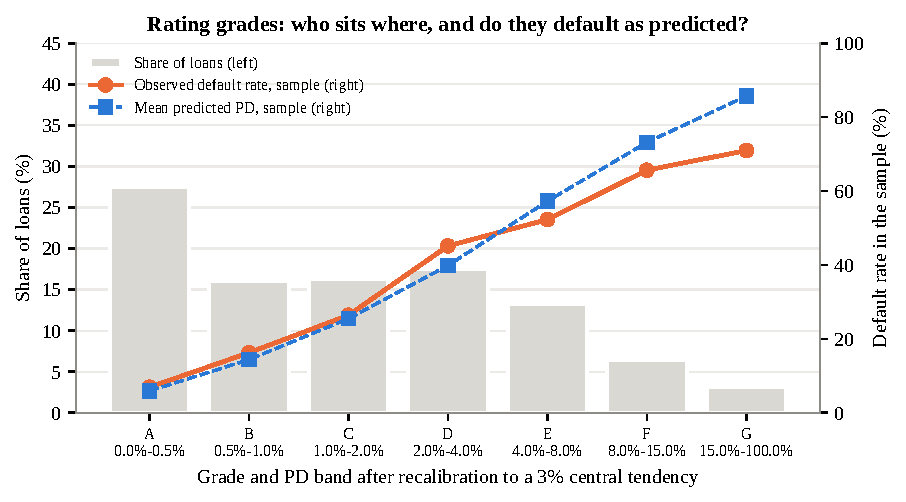
\includegraphics[width=0.80\textwidth]{../figures/fig5_grades.pdf}
\caption{Rating grades: share of loans, observed and predicted default rates (paper, Figure 5).}
\coderef{notebooks/german\_credit\_risk.ipynb, cell [13] (matplotlib, twin axes)}
\end{figure}

\section{Step 7: translating PDs into regulatory capital}
The capital formula of the CRR for retail exposures is short enough to write in a few lines, and writing it myself was the best way to understand it. \texttt{norm.ppf} and \texttt{norm.cdf} are the inverse and the cumulative standard normal distribution from SciPy; the PD floor of 0.05\% introduced by CRR3 is applied first.

\par\noindent\begin{minipage}{\linewidth}
\lstinputlisting[style=py,firstline=25,lastline=42,firstnumber=25]{../src/irb.py}
\coderef{src/irb.py, functions other\_retail\_correlation(), capital\_k(), risk\_weight()}
\end{minipage}\par

Because the functions are vectorised with NumPy, the same code computes the risk weight of one loan, of 1,000 loans, or of 300 points along a curve for the chart. The notebook then aggregates risk-weighted assets, expected loss and the output-floor test, and repeats the calculation for six combinations of PD and LGD.

\begin{figure}[H]\centering
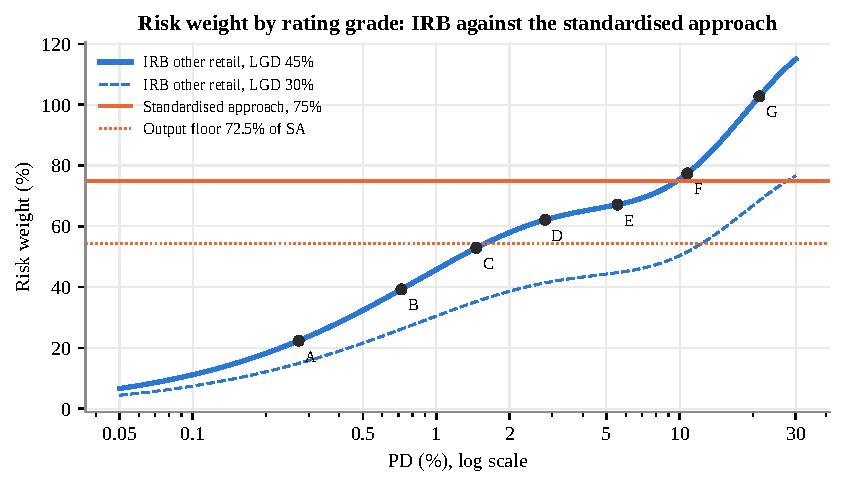
\includegraphics[width=0.80\textwidth]{../figures/fig6_risk_weights.pdf}
\caption{IRB risk weight by grade against the standardised approach (paper, Figure 6).}
\coderef{notebooks/german\_credit\_risk.ipynb, cells [14] (capital), [15] (sensitivity), [16] (chart) \textbar{} src/irb.py}
\end{figure}

\section{Step 8: reporting and reproducibility}
The last cell exports five CSV files to \file{outputs/}: one row per loan with PD, grade, risk weight and expected loss, plus summaries by grade, the model comparison, the Information Values and the capital sensitivity. They are shaped for a Power BI report: one fact table and four small summary tables that Power BI can read straight from the folder, so the report refreshes whenever the notebook is run again.

\par\noindent\begin{minipage}{\linewidth}
\begin{lstlisting}[style=py]
port.to_csv(OUT / "scored_portfolio.csv", index_label="loan_id")
cols = ["rw_irb", "el_pct", "exposure_share"]
g.join(by_grade[cols]).to_csv(OUT / "grade_summary.csv")
res.to_csv(OUT / "model_comparison.csv")
iv_tab.to_csv(OUT / "information_values.csv")
sens.to_csv(OUT / "capital_sensitivity.csv", index=False)
\end{lstlisting}
\coderef{notebooks/german\_credit\_risk.ipynb, cell [17]}
\end{minipage}\par

The two modules are covered by unit tests in \file{tests/}. They check the risk weight against a value worked out by hand from the CRR formula, that the PD floor is applied, that recalibration hits its target without changing the ranking, that a pure-noise variable gets an Information Value close to zero, and that categories or values never seen in training do not break the encoder. A GitHub Actions workflow runs them on every push. The whole project can be rebuilt from the command line:

\par\noindent\begin{minipage}{\linewidth}
\begin{lstlisting}[language=bash,numbers=none]
pip install -r requirements.txt pytest
pytest -q
jupyter nbconvert --to notebook --execute --inplace notebooks/german_credit_risk.ipynb
Rscript R/pd_logit.R
\end{lstlisting}
\coderef{README.md, section ``How to run''}
\end{minipage}\par

\section{What I would do differently}
The project has clear limits, and some of them are programming choices I would change with more time.

\begin{itemize}[leftmargin=1.5em,itemsep=2pt]
\item \textbf{More tests.} The modules are tested, the notebook is not. I would move the model-comparison loop into a function and test it on a small synthetic dataset.
\item \textbf{Hyperparameter tuning.} The random forest and the gradient boosting model use reasonable defaults. A grid search inside the cross-validation would make the comparison with the scorecard stricter, although with 1,000 loans I do not expect a large change.
\item \textbf{Data pipeline.} The system-level data are collected by hand. With API access, a script could download the ECB and Bundesbank series directly and update the charts on a schedule.
\item \textbf{Better data.} Re-running everything on the corrected South German Credit data would remove the known labelling problems.
\end{itemize}

\medskip
\textit{The paper, the notebook and all the code referenced here are in the project repository.}

\end{document}
